\section{Nouveauté}
	
	Les principales nouveauté trop cool de notre logiciels....	Aliquam finibus est ac cursus cursus. Fusce in libero ut nisi laoreet sodales. Cras vestibulum nec nulla in consequat. In eget lacus ut ipsum placerat ultrices. Nam diam magna, fermentum aliquam libero at, ornare eleifend diam. Sed et mi eget arcu bibendum congue. Vivamus in enim mollis, blandit sem in, hendrerit tellus.


	\subsection{Optimiseur}

		Mauris rhoncus tempor rhoncus. Vestibulum lacinia tincidunt sem ac auctor. Maecenas a lectus in nisi aliquet feugiat. Sed gravida laoreet maximus. Donec feugiat vestibulum neque sit amet mollis. Maecenas commodo luctus augue et molestie. Maecenas viverra semper massa, blandit commodo lacus blandit a. Proin sed euismod massa. Aenean nec nisl sed nisi mollis congue quis a nisi. Pellentesque habitant morbi tristique senectus et netus et malesuada fames ac turpis egestas. Suspendisse tincidunt euismod ipsum vitae commodo. Ut dapibus tellus nec libero egestas, eu venenatis dolor fermentum. Donec porttitor erat ante, at tincidunt lacus efficitur vitae.

		Vivamus elit urna, suscipit et nisi in, semper fringilla elit. In euismod cursus nunc quis tincidunt. Phasellus efficitur eleifend lacus, et pellentesque risus rhoncus vel. Phasellus in euismod lorem. Nam pulvinar aliquam metus a scelerisque. Etiam eget lectus ut felis porta ullamcorper. Aenean commodo at augue id pulvinar. Nunc efficitur elit est, id placerat sapien sodales nec. Etiam finibus at lacus nec viverra. Integer at vulputate mauris. Maecenas eget magna id tellus imperdiet finibus et in purus. Integer placerat ipsum a dui pellentesque, in lobortis lorem lobortis. In hac habitasse platea dictumst. 

	\subsection{Filtre}
		\begin{figure}
			\begin{center}
				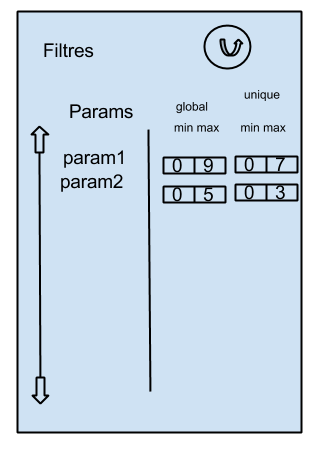
\includegraphics[width=0.25\textwidth]{figure/filtre.png}
			\end{center}
			\caption{Filtre}
			\label{fig:filtre}
		\end{figure}


		\begin{itemize}
		  \item bouton pour ajouter nouveau paramètre sur le filtre (par default : pas de filtre => pas de paramètres) 
			  \begin{itemize}
			  	 \item ajouter ouvre selection de paramétres : menu déroulant précisant les paramètres disponibles.
			  \end{itemize}
		  \item tous les paramètres ont à coté d’eux deux sections : une de filtre global et une de filtre unitaire. Dans le filtre global sont présentes deux cases, une nommée “min” et une nommée “max”. De même dans le filtre unitaire.
		  \item par défaut, les min sont moins l'infini et les max sont l’infini (pas de filtre)
		  \item il est possible d’inscrire des valeurs dans les cases “min” et “max” afin de réduire l’intervalle de sélection des branches de l'arbre.
		  \begin{itemize}
			  	 \item la section globale permet de conserver les branches de l’arbre dont la valeur totale du paramètre se trouve dans l’intervalle. (ex : entre 500 et 1000 euros au total)
			  	 \item la section unitaire permet de conserver les branches de l’arbre dont chacune des valeurs de chacune des feuilles se trouve dans l’intervalle. (ex : pas de dépenses de moins de 10 euros et pas de plus de 100 euros)
		  \end{itemize}
		  \item il est ainsi possible de combiner les critères de sélection (ex : entre 500 et 1000 euros au total et pas de dépenses de moins de 10 euros et pas de plus de 100 euros ; et le temps entre X et Y et ….)
		  \item barre de défilement pour les cas de surcharge de paramètres
		  \item possibilité d'activer ou désactiver les paramètres ( bouton a cocher)
		  \item bouton ``générer'' permet de créer un nouvelle arbre filtré en fonction des paramètres définie. Il est ouvert dans un nouvelle onglet de la section ADTool de l'interface. 
		  \item chaque arbre posséde son propre outil filtre. Lors de la génération, le nouvelle arbre posséde un outil filtre vide. 
		  \item le nouvel arbre posséde un commentaire : filtre depuis l'arbre X avec paramétre Y, heure, version. \ldots
		  \end{itemize}


	\subsection{Fonction de synthése}
		\begin{figure}
			\begin{center}
				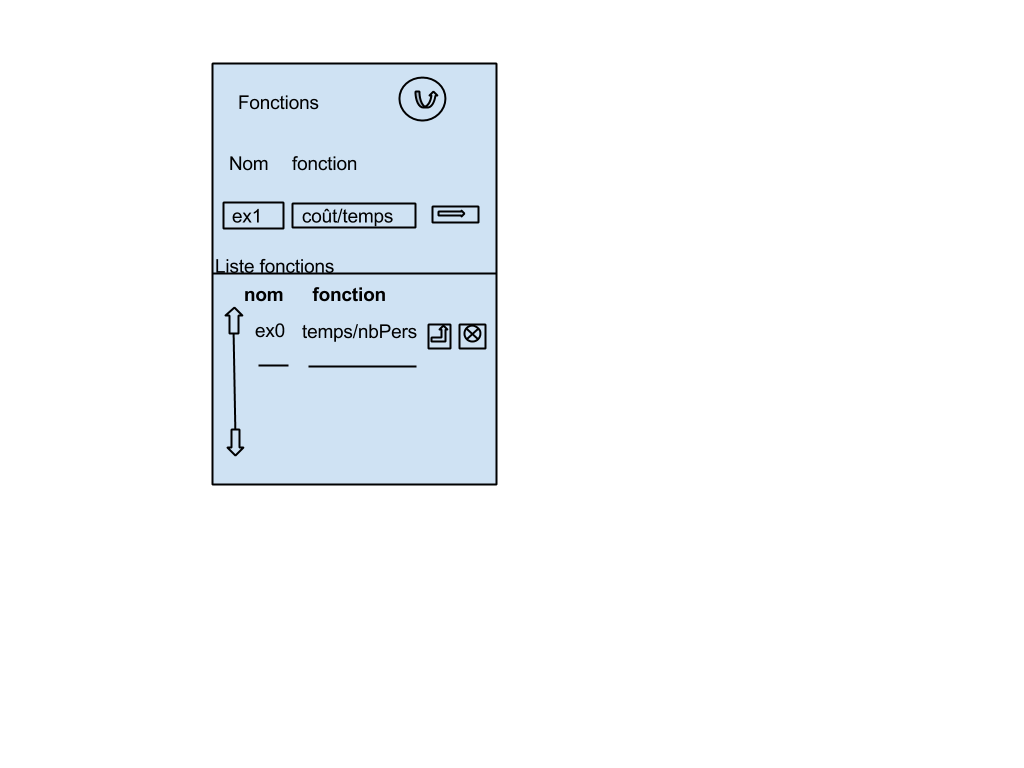
\includegraphics[width=0.25\textwidth]{figure/fonction.png}
			\end{center}
			\caption{Fonction}
			\label{fig:fonction}
		\end{figure}

		\begin{itemize}
			\item (présence préallable de 6 valuations de synthèse définies dans ADTool, et non instanciées par défaut. )
			\item décomposition en deux zones : une pour l'édition du nouveau paramètre et de sa fonction, et une pour le rappel des fonctions déjà existantes.
			\item Zone 1 : Présence d’un menu déroulant pour choisir laquelle des 6 valuation de synthèse est à instancier, et d'une zone textuelle pour écrire la fonction qu'on lui associe. La fonction est une fonction linéaire ou non, et qui prend en paramètres des valuations de l'arbre déjà définies (dans ADTool ou d'autres fonctions de synthèse). Bouton à coté pour valider la création. Si echec de la création (fonction non valable, etc.), message d'erreur donné par le guide (avec conseils éventuels).
			\item zone 2 : présence en dessous de la zone 1 d’une zone de rappel des fonctions de synthèse déjà instanciées. A coté de chacune d’entre elles il y a deux boutons : un pour modifier une fonction déjà créée, et un autre pour la supprimer.
			\item bouton “actualiser” en haut pour mettre à jour la liste des fonctions. \ldots
		\end{itemize}
		
		
		

